\documentclass[../main/main.tex]{subfiles}


\begin{document}

\section{April 11th, 2019}
\subsection*{Review}
\begin{itemize}
	\item At each iteration, the algorithm picks exactly one edge.
	\item The edges picked form a forest $F$.
	\item Active component are those that belong to $S^{\star}$.
	\item If $F$ is not primal feasible, then there must be some connected component in $F$ that is unsatisfied (active).
	\item We raise the dual simultaneously for all active components in a synchronized manner until some edge goes tight.
	\item We pick one of the edges and merge such components, terminating the iteration.
	\item We stop when a primal feasible solution $F$ is formed (no active components).
\begin{figure}[h!]
	\centering
	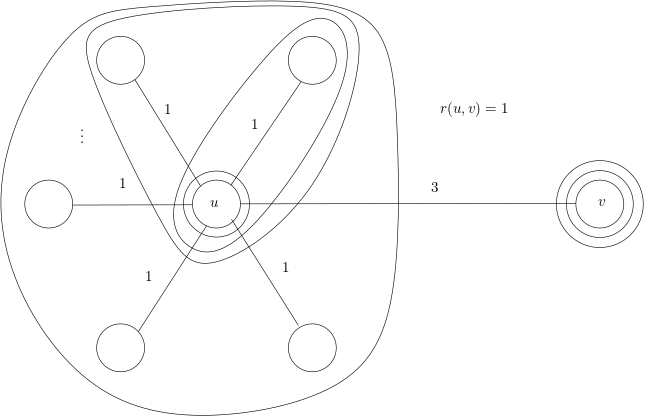
\includegraphics[width=0.8\textwidth]{4-11-spokes}
\caption*{Dual: $2+1=3$}
\caption*{Cost of solution: 3 + 1$\times $\# of spokes =  $3+(|V|-2=|V|+1=\Omega(|V|)$}
	\label{fig:4-11-spokes}
\end{figure}
\item As shown above, the solution might give us a terrible approximation ratio, which is why we have a pruning step to drop the redundant edges. After doing so, we would have cost of solution = 3.
\item This can be done by seeing if $F-\{e\} $ satisfy the connectivity constraints, removing it if it is redundant. This will give us $F'$. 
\end{itemize}
\subsection{Steiner Forest Algorithm Correctness and Approx. Ratio}
\begin{itemize}
	\item\textbf{Correctness} - At termination, dual is feasible and primal is feasible. 
	\begin{proof}
		\begin{itemize}
			\item Dual is feasible because as soon as the dual constraint goes tight, the dual variable is frozen and thus the edges do not become over-tight.
			\item Primal is feasible because:
				\begin{enumerate}
					\item Before the pruning step, the primal solution obtained is feasible (we stop only when all constraints of $F$ are satisfied.
					\item The pruning step does not hurt feasibility. Note that for each pair of vertices $u,v$ that have a connectivity constraint ($r(u,v=1$), there is a unique path between the two in $F$. Each edge $e$ on that path will not be removed, as $u,v$ would not be connected. 
				\end{enumerate}
		\end{itemize}
	\end{proof}
\item\textbf{Approximation Ratio} The approximation ratio of this algorithm is $2$.
	\begin{proof}
		\begin{itemize}
			\item By weak duality, \[
			\sum\limits_{S\in S^{\star}} y_s \le OPT
			,\] where $OPT$ is the cost of the optimal Steiner Forest.
		\item Note: \[
				\sum_{S\in S^{\star}}y_s=\sum_i \left(\Delta_i\times \text{\# of active components}\right)
			,\] where $\Delta_i$ is the amount by which the duals of each active components is raised on the $i$-th iteration. (try to do this without using LP-duality)
		\item Now we'd like to show that $Cost(F')\le 2\times \sum\limits_{S\in S^{\star}}y_S\le 2\times OPT$.
		\item Let us define: \[
				\text{Degree of $S\subseteq V$}:= \# \text{ of edges in $F'$ that belong to the cut $(S,\overline{S})$}
			.\]
			\begin{figure}[h!]
				\centering
				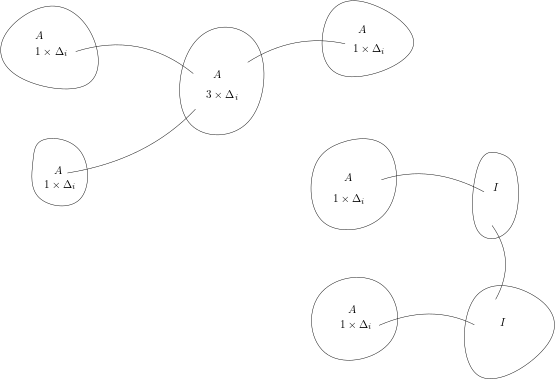
\includegraphics[width=0.55\textwidth]{4-11-di}
				\label{fig:4-11-di}
			\end{figure}
		\item The above diagram demonstrates that: \[
				Cost(F')=\sum_i\left( \Delta_i\times \sum_{S \text{ is active}}\text{Degree of $S$}\right) 
		.\] 
	\item Suppose that $\text{Degree of $S$}\le 2$, we would have our approximation ratio. (however this is not true, as shown above).
	\item Consider the average:\[
Cost(F')=\sum_i\left( \Delta_i\times \sum_{S \text{ is active}}\text{Degree of $S$}\right)\]\[
=\sum_i\left( \Delta_i\times \text{\# of active components} \times \text{Average Degree of active components}\right)
.\]  meaning we have to show that the average degree of active components is less than or equal to 2.
	\item For a tree, it has $n$ vertices and $n-1$ edges, meaning that average degree = $\frac{2(n-1)}{2}\le 2$. So this is true for a forest.
	\item As such, if all components are active, then we are done, however this is not true in general, as an active component might have many inactive components connected.
	\item However, due to the pruning step, all inactive components must be internal.
	\item Consider the simple case first. Suppose there were no inactive components in iteration $i$. The average degree of the active components $\le$ average degree of a tree $ \le 2$.
	\item If there are inactive components that are leaves, we might be in trouble, as they would have degree 1, meaning that the average degree of active components could be $\ge 2$.
	\item However, the clearly cannot be the case because of the pruning step.
	\item Thus any inactive component must have degree $\ge 2$ as they are internal, meaning that the degree of active components $\le 2$.
		\end{itemize}
		\begin{remark}
			What if an inactive component has degree 0? (only consider the connected components with active component) TODO: think about this more
		\end{remark}
	\end{proof}
\end{itemize}
\end{document}

